Protein coding genes have dominated the study of genetics for decades. The rules by which they function are well understood and we can often predict the function of an unknown gene based off of its underlying sequence content. This is due to the well understood rules of protein coding reading frames and the principles of conservation in biology. In the early 1990s (get actual date), an RNA transcript was discovered that was essential for the process of X chromosome inactivation (XCI), by which an entire X chromosome in female eutherians is near completely transcriptionally silenced. This transcript, known as Xist, does not code for protein, but rather is a non-coding RNA.

The advent of RNA sequencing has led to an explosion of annotated RNA transcripts that have no corresponding protein products. Even with numerous advances in genetics and genomics, these RNAs have proven to particularly challenging to understand. 
\section{Long non-coding RNAs}
Long non-coding RNAs (lncRNAs) are defined as non-coding RNA transcripts longer than 200 base pairs (bp). lncRNAs have emerged as a major mechanism of gene regulation in eutherians, however they have been annotated in all eukaryotic organisms. Humans in particular have many thousands of annotated lncRNAs, but the overwhelming majority have no known functional role, if any. Despite this, it is known that several lncRNAs play key roles in differention, development, as well as disease. 

Of the lncRNAs that have been studied and have known function within the cell, there often is considerable work left to fully understand the function of these transcripts, despite many years worth of work. A particular challenge with lncRNAs is that they are often poorly conserved related to protein coding genes, if they are conserved at all. Furthermore, conventional alignment tools such as BLAST or nhmmer fail to detect meaningful relationships between two transcripts with similar function. 

lncRNAs are difficult to study experimentally, as well. lncRNAs rarely function in isolation, but rather through the concerted action of the lncRNA transcripts, RNA binding proteins, and other biological molecules such as DNA or other proteins. This indicates that lncRNAs exist in a complex network of interactions that has proven difficult to unravel. 
\subsection{Functional annotation}
Long non-coding RNAs biochemically are very similar to mRNAs, in fact there is very little other than the presence of a reading frame that differentiates an messenger RNA from a lncRNA. lncRNAs are thus genes for which the final functional product is an RNA transcript. Given that RNA molecules are known to chemically bind to numerous biological molecules, including protein, DNA, and RNA itself, it perhaps comes as little surprise that lncRNAs are capable of widely varied function within the cell. 

lncRNAs have generally been grouped into several sub-categories based on broadly defined features of their loci. The primary groups that have been annotated are intergenic lncRNAs (lincRNAs), which are found between annotated protein coding genes, anti-sense lncRNAs, whose loci are located on the anti-sense strand relative to a known gene, and intronic lncRNAs, which are encapsulated within the intron of a protein coding gene. The vague and non-specific nature of these definitions underlines how little is known about lncRNAs in general. In comparison, we can annotate protein coding genes down to their exact roles within the cell, not-with-standing larger classifications into cliques and communities within larger functional networks. 

What is relatively well known is that lncRNAs are often involved in genetic regulation. Since the discovery of \emph{XIST} and the further identification of additional lncRNAs in years following the introduction of next generation sequencing, it has become clear that a primary functional role of lncRNA is the regulation of gene expression in human and other mammalian genomes. While RNA-seq has allowed for the rapid discovery of genes that produce RNA transcripts as their final product, the elucidation of the function for these newly annotated transcripts has proven far more challenging. 

\subsubsection{Guilt by association}
Assigning functional roles to lncRNAs, if there is any function to be assigned, has proven to be a daunting task. One of the first methods used is the so-called \emph{guilt by association} hypothesis. Rather than trying to identify the specific function of a lncRNA, trends from gene expression data are used to attempt identify features such as specificity of cell type expression. A more advanced approach uses informatics techniques to identify protein coding genes and biological pathways that are co-regulated with specific lncRNAs, with the underlying assumption that if a lncRNA is co-regulated with a specific pathway, it is likely to have a functional role within that pathway. 

This methodology is useful for identifying transcripts that may be useful for further targeted experimental studies, but \emph{guilt by association} is an inherently correlative method that does provide real insights into the lncRNAs of interest. Despite this shortcoming, several functional lncRNAs have been identified and characterized this way. 

\subsubsection{High throughput loss of function screens}
Perhaps the holy grail of lncRNA functional annotation is a reliable high throughput screening methodology to ascribe function to lncRNA transcripts. RNA interference studies have found that lincRNA knockdowns can have profound effects throughout the transcriptome, especially in the maintenance of stem of cells. RNAi screens suffer from several limitations, however, including variance in silencing and off-target effects. Within the realm of cancer biology, RNAi screens have led to several well known examples of erroneously ascribed function, including \emph{MELK} and \emph{STK33}.

Traditional \emph{CRISPR} approaches are not viable as lncRNAs lack reading frames, however over- and under-expression extensions such as \emph{CRISPRa} and \emph{CRISPRi} have identified functional lncRNAs (\citep{Cai2020AHomeostasis}). Despite these successes, the correlative nature of these screens are just the first steps in elucidating the mechanisms by which a lncRNA function. 

Of the small number of lncRNAs that have well characterized roles within the cell, many still have their exact mechanism of action being actively studied. \emph{XIST} is one of the most well known lncRNAs and was discovered in the early 1990s, however there is still considerable controversy about how exactly it enacts XCI. \emph{XIST} serves as a reminder that these genes are very complicated and are often multi-faceted in their function, and so therefore there remains a massive amount of work left in the field to sift through the truly enormous number of annotated lncRNAs in the human genome.

\subsection{lncRNA mediated gene regulation}

The connection between RNA and chromatin has long been known. Early chromatin purification experiments revealed that potentially twice as much RNA as DNA associated with chromatin. Further studies have shown that several lncRNAs, such as \emph{XIST}, \emph{AIR}, \emph{KCNQ1OT1}, and others associate with chromatin and modulate the deposition or removal of regulatory markers on chromatin. 

One feature shared by all these transcripts is the formation of RNA-protein complexes, often involving numerous RNA binding proteins at several different regions within the lncRNA transcript. 

\section{Xist as a model lncRNA}
The XIST lncRNA is one of the most well characterized lncRNAs due to its essential role in XCI and because it is one of the few transcripts that is completely conserved in all eutherians. XCI is the process by which mammalian females transcriptionally silence a single X chromosome as a means of gene dosage compensation. Proper expression of Xist is required for initiation of XCI, and XIST is required for silencing virtually all genes on the inactive-X. While X-inactivation is complex, involving many additional factors beyond XIST, and mechanistic details are still an area of active research, XIST provides a well-studied example of lncRNA activity.

Given that Xist is one of the only well known lncRNAs, and that its function is approximated in other functional analogs in the human and mouse transcriptomes, such as the lncRNAs AIRN and KCNQ1OT1, XIST will be used as a ground truth approximation for the rules by which cis-acting repressive lncRNAs function.

\section{$k$-mer based sequence comparison}
Traditional pairwise alignment has been a mainstay of bioinformatics for decades. Originally for detection of homologous sequences, pairwise alignment is now crucial for next generation sequencing experiments. A fundamental issue with pairwise alignment is its complexity. To obtain the best alignment between $N$ sequences of length $L$, $L^N$ calculations have to be made. To compare just 5 sequences of 100bp each, $10^{10}$ calculations would have to be made! For this reason, expedients have long been sought. Alignment-free methods of sequence comparison have existed almost as long as sequence alignment has.

A particularly common form of alignment-free comparison involves $k$-mer frequency comparisons. A $k$-mer is defined as a sub-sequence of length $k$ within a larger sequence. $k$-mer based methods have been used for a variety of purposes, but most commonly for examining speciation in metagenomic samples and the evolutionary distance between two species. For DNA, as the value of $k$ is increased, the number of possible permutations of the four nucleotides increases exponentially ($4^k$). Therefore, the amount of shared overlap of $k$-mers is a function of their evolutionary distance from each other. Closely related species may show significant overlap for $k\in[14,26]$, whereas distantly related species may have the same amount of overlap for signficantly smaller values of $k\in[8,12]$.

These methods are based on the frequencies of $k$-mers within a larger sequence, not on direct alignment between two sequences. Therefore statistics can quickly be calculated that quantify the degree of similarity between two sets of $k$-mers. However, as described above these methods have been traditionally applied to evolutionary relations, and not as a functional model of sequence content. 

Our lab has recently developed a $k$-mer based method for assessing functionality in long non-coding RNAs. In the following section the motivation and algorithm for using $k$-mers to predict functionality in long non-coding RNAs will be described. 

\subsection{SEEKR Algorithm}

 While the sequence relationship between functionally analogous lncRNAs is undetectable with traditional alignment tecniques, their sequences are not random. We hypothesized that lncRNAs with shared functions must contain some sequence similarity that confers the shared function, even if conventional alignment algorithms do not detect the similarity. Many of the known and well studied lncRNAs function through the recruitment of RNA binding proteins, or RBPs. These proteins are highly conserved and recognize short, 4-6bp motifs on an RNA strand. lncRNAs are further differentiated from protein coding genes in that they do have reading frames -- such that we expect that motifs for RNA binding proteins may be located anywhere in a sequence and still recruit that protein. These observations of lncRNA functionality led us to develop a $k$-mer based bag-of-words model for the sequence-to-function relationship in lncRNAs.
 
 \begin{figure}[t!]
\centering
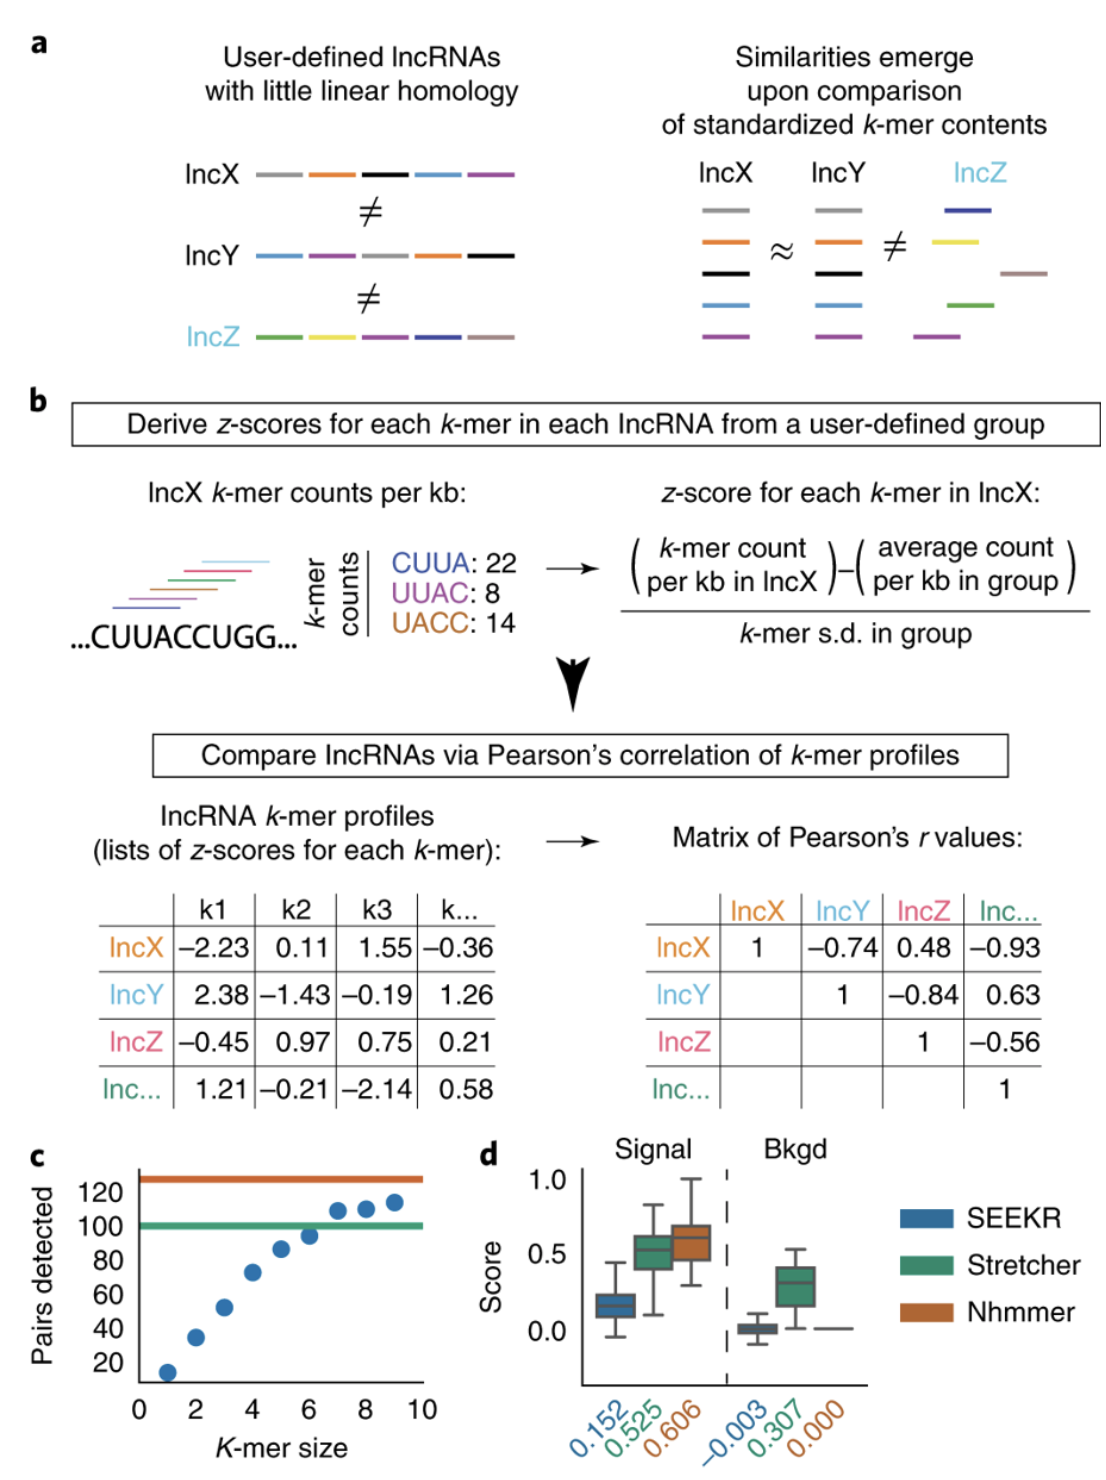
\includegraphics[width=.8\textwidth]{images/seekr.png}
\caption[width=.8\textwidth]{(A) LncRNAs of related function (names in black) may harbor similar sequence similarity in the form of motif content (colored bars) even if they lack linear homology. (B) In SEEKR, the abundance of all kmers of length k are counted by tiling across each lncRNA in a user-defined group in one nucleotide increments.}
\label{fig:seekr}
\end{figure}

Our lab developed an algorithm for comparing $k$-mer content between lncRNAs, called SEEKR (SEquence Evaluation from Kmer Representation). Within the algorithm, each $k$-mer in a sequence is counted through a 1bp sliding window. $k$-mer counts for each lncRNA are then normalized by lncRNA length and standardized across a reference set (\emph{e.g.} the transcriptome) to derive a matrix of standardized $k$-mer frequencies. The degree of similarity between two lncRNA transcripts can then be calculated using the pearson correlation coefficient.


\section{Hidden Markov Models}
A hidden markov model (HMM) is a generative probabilistic model for stochastic sequential processes. For some observable process, or sequence, $X$, we assume there is an underlying random process $Y$ that is controlling the behavior of $X$. A generative probabilistic model such as an HMM calculates the joint probability distribution $P(X,Y)$, rather than the more commonly seen classifier, or discriminative model, that models the conditional probability distribution $P(Y|X)$ such that a most probable classifier label can be assigned to $X$.

The reason for modeling the joint distribution $P(X,Y)$ is that it allows an HMM to not only calculate the probability of any given sequence, but allows for the generation of randomized outcomes of the model. HMMs therefore reflect a simplified, hypothesized process by which the data may be reasonably generated.

To allow for tractable calculation of probabilities, an HMM relies on the Markov assumption, which posits that the current observation is conditionally independent of all other observations, except for the observation immediately prior. This assumption is formally defined in Equation \ref{eq:markov}.

\begin{equation}
    P(x_t|x_{t-1},x_{t-2},\dots,x_1) = P(x_t | x_{t-1})
\label{eq:markov}
\end{equation}

This assumption appears simplistic, but it is often sufficient for many modeling tasks that would be impossible without simplifying assumptions. HMMs have been used in many fields, from weather prediction to text prediction, such as a common search engine query \emph{e.g.}: 

\begin{center}
    $P(\texttt{park} | \texttt{dog,nearest,the,where's}) > P(\texttt{office} | \texttt{dog,nearest,the,where's}) $
\end{center}

Could be accurately modeled with the markov assumption:

\begin{center}
    $P(\texttt{park} | \texttt{dog}) > P(\texttt{office} | \texttt{dog}) $
\end{center}

A markov based model would be able to reliably suggest the word \emph{park} instead of \emph{office} because the word \emph{office} would almost never follow the word \emph{dog}, regardless of the remainder of the sentence. This assumption has proven to be wildly useful in the field of bioinformatics, especially with probabilistic modeling of DNA sequences. Mammalian chromosomes can be hundrends of millions of basepairs long, but in reality the relationships between nucleotides exist on much shorter scales. Often a nucleotide can be accurately predicted from preceeding sequence using only the previous 5-6 nucleotides (GENSCAN).

\subsection{Gene finding and other applications}
HMMs have been used for many purposes, from sequence alignment to modeling the timing of switches in fluorescence from FRET experiments. An early application of HMMs to biological data was gene finding in the 1990s. During this period the Human Genome Project was well underway, and only a fraction of protein coding genes were known. Huge regions of the human genome were being sequenced but massively parallel RNA sequencing technology did not exist at the time, so it was unknown where genes were in the human genome. Therefore, computational models were developed to predict regions within the genome that contained reading frames. 

The majority of the methods developed utilized HMMs at their core. The reason for this was relatively straightforward. Protein coding genes are composed of distinct functional domains, and each of these functional domains contains their own unique nucleotide distributions. Therefore, we can start with a very general model of protein coding gene:

\begin{center}
    Promoter$\rightarrow$5' UTR$\rightarrow$Exon$\rightarrow$Intron$\rightarrow \dots \rightarrow$ 3' UTR
\end{center}

Using the nomenclature defined in 1.4.1, this is the sequence of hidden states $Y$. The actual DNA sequence that we observe,$X$, is controlled by the presence of these functional domains, and an HMM calculates the joint probability of the parse of the sequence $Y$ and the sequence $X$, or $P(X,Y)$. The idea is that some parses will be more likely than others, and that we can then use this model to identify the most likely parse $Y^*$ of the data. 
\begin{figure}[h]
\centering
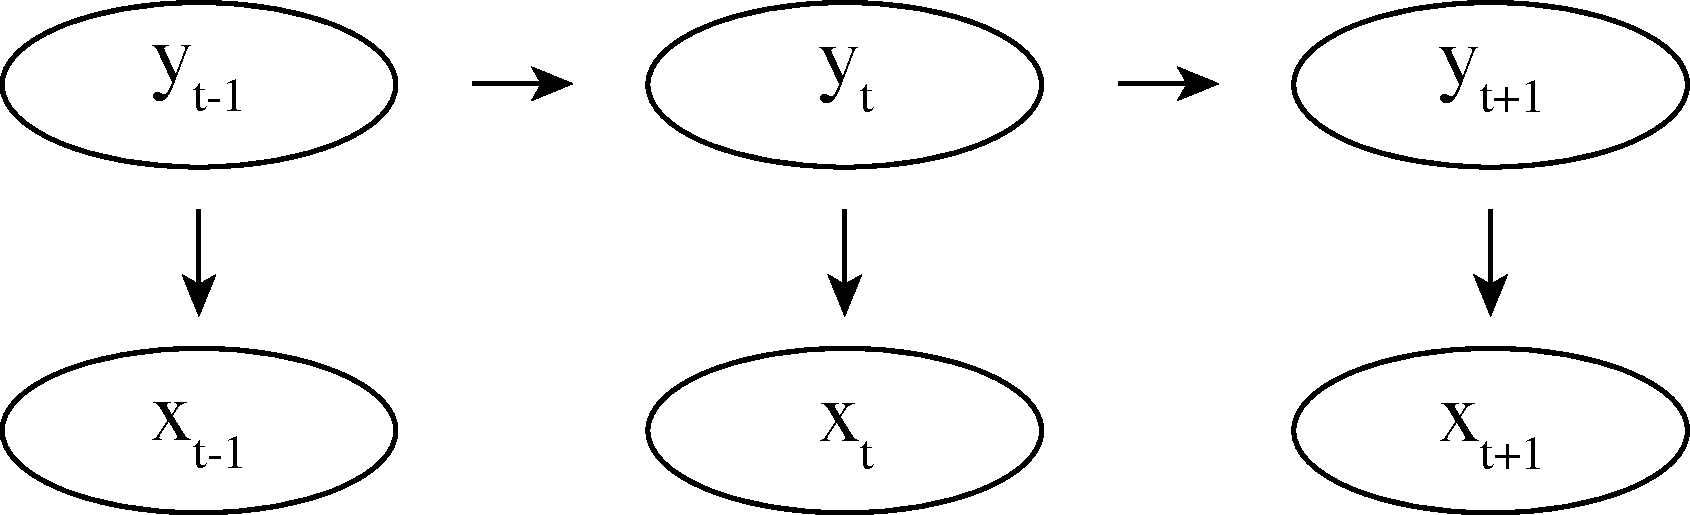
\includegraphics[width=\textwidth]{images/hmm.pdf}
\caption{Conditional dependencies in a hidden markov model.}
\label{fig:HMM}
\end{figure}
\subsection{Model structure}
The HMM is constructed with the Markov assumption placed on the sequence of hidden states $Y$, so that for a sequence of length $L$ the probability of the current hidden state $y_i$ is dependent only on the previous hidden state $y_{i-1}$. Further, $y_i$ does not depend on the observed sequence $X$. 
\begin{equation}
    P(y_t,X_{1:L},Y_{1:t-1},Y_{t+1:L}) = P(y_t|y_{t-1})
\end{equation}

And the probability of each observation $x_i \in X$ is conditionally independent of everything except the emitting state at time $i$, $y_i$, and is not dependent on any other $x_{j,j\neq i} \in X$.

\begin{equation}
    P(x_t,X_{1:t-1},X_{t+1:L},Y_{1:L}) = P(x_t|y_t)
\end{equation}

These conditional independencies can be represented in the graphical form illustrated in Figure \ref{fig:HMM}. 

From here the joint probability for an HMM can be derived. This explicitly allows the calculation of the probability for all possible sequences of observations and all possible sequences of hidden states. 

\begin{equation}
    P(X,Y) = P(y_1)p(x_1|y_1)\prod_{t=2}^L{P(y_t|y_{t-1})P(x_t|y_t)}
\label{eq:jointhmm}
\end{equation}

This joint probability distribution allows us to work with the three most common tasks that HMMs are used for: evaluation, decoding, and learning.
\subsection{Inference and Algorithms}
There are three primary questions that an HMM is used to answer. 

\begin{enumerate}
    \item Evaluation: What is the probability of being in a given state, at a particular point in time? A related quantity is the total probability of the observed sequence, \emph{i.e.} $P(X)$. This value is crucial from converting the joint distribution to conditional distributions, especially with respect to Baye's Theorem and the calculation of maximum likelihood estimates for parameters.
    \item Decoding: What is the most likely parse of the sequence? 
    \item Learning: What are the most likely set of parameters, given the observed data?
\end{enumerate}

\subsubsection{Combinatorial Explosion}
To answer the above questions through complete enumeration over all possible combinations of observed sequences and the corresponding possible sequences of hidden states, $K^L$ combinations would have to explored, where $L$ is the length of the sequence and $K$ is the number of hidden states. For an average gene of $L=1000$bp and 5 hidden states, $5^{1000}\approx10^{698}$, total calculations would have to be made. This is clearly intractable, even for far shorter sequences. Fortunately algorithms have been developed that make these calculations linear with respect to the length of the sequence.
\subsubsection{Observation Likelihood}
A key quantity when working with HMMs is the total likelihood of the observed sequence $P(X)$. Specifically, we want to know the probability of the observed sequence over \emph{all possible parses} $\phi_i \in \Phi$. Here $\Phi$ refers to the set of all possible parses, and $\phi_i$ refers to an individual parse selected from $\Phi$. 

\begin{equation}
 P(X) = \sum_{\phi_i \in \Phi}{P(X,\phi_i)}  
\label{eq:partition}
\end{equation}

To make it more clear what this quantity is, an example is provided. Let $X = ATC$, and let the set of hidden states be simply $\left\{0,1\right\}$. The set of \emph{all possible parses} $\Phi$ is then a set of $2^3$ elements:

$$\Phi = \{\{000\},\{001\},\{010\},\{011\},\{100\},\{101\},\{110\},\{111\}\}$$

A randomly chosen parse $i$ from this set, $\phi_i \in \Phi$ could be

$$\phi_i = \{010\}$$

Using equation \ref{eq:jointhmm}, there is a joint probability of observing $X=ATC$ and $Y = \phi_i = 010$.

$$P(X=ATC,Y=010)$$

Given that X is fixed, there are still 7 other joint probabilities for each of the remaining possible parses

$$P(X=ATC,Y=000)$$
$$\vdots$$
$$P(X=ATC,Y=111)$$

The law of total probability (Eq. \ref{eq:totalprob}) states that, for two random variables $A$ and $B$ with a joint distribution $P(A,B)$ the marginal distribution $P(A)$ can be calculated by summing over all possible values of $B$.

\begin{equation}
    P(A) = \sum_B{P(A,B)}
\label{eq:totalprob}
\end{equation}

Within the context of our HMM, we are interested in knowing the probability of our observation $X=ATC$ regardless of the actual parse. To do this, we apply equation \ref{eq:totalprob} and sum each of the joint probabilities above to get the probability that $X=ATC$, yielding equation \ref{eq:partition}.

This quantity is important for several reasons, but as described above is impossible to calculate through a brute force approach, as the size of the set $\Phi$ combinatorally explodes.

Fortunately, there exists an algorithm which can efficiently calculate $P(X)$ with a computational complexity of $LK^2$, compared to the $K^L$ complexity described above.
\subsection{Forward and Backward Algorithms}
\subsubsection{Forward Algorithm}
The forward algorithm recursively calculates the total probability of the sequence $X$ starting from the first observation. This calculation is made feasible by using the conditional independencies demonstrated in Figure \ref{fig:HMM} and the joint probability distribution in equation \ref{eq:jointhmm}.

\subsubsection{Initialization}
\begin{equation}
    \alpha_i(t) = p(x_1|y_i)p(y_i)
\label{eq:fwdinit}
\end{equation}

\subsubsection{Induction}
$2\leq t\leq L$
\begin{equation}
    \alpha_i(t) =p(x_t|y_i)\sum_{j}{p(y_i|y_j)\alpha_j(t-1)}
\label{eq:fwdinduc}
\end{equation}

\subsubsection{Termination}
\begin{equation}
    P(X)= \sum_i{\alpha_i(t=L)}
\label{eq:fwdterm}
\end{equation}

Here $i$ and $j$ are an element in the set of hidden states. The final term, summed over all hidden states, represents the total probability of the observed sequence $X$.

\subsubsection{Backward Algorithm}
The backwards probability $\beta$ is the probability of seeing the observations from time t + 1 to the end, given
that we are in state i at time t.

\subsubsection{Initialization}
\begin{equation}
    \beta_i(t=L) = 1
\label{eq:bwdinit}
\end{equation}

\subsubsection{Induction}
$T-1\leq t\leq 1$
\begin{equation}
\beta_i(t-1) =p(x_{t-1}|y_i)\sum_{j}{p(y_i|y_j)\beta_j(t)}
\label{eq:bwdinduc}
\end{equation}

\subsubsection{Termination}
\begin{equation}
    P(X)= \sum_i{\beta_i(t=1)} = \sum_i{\alpha_i(t=L)}
\label{eq:bwdterm}
\end{equation}

The forward and backward algorithms can be combined to calculate the probability of being in any hidden state $i$ at any position within the sequence, \emph{i.e.} $P(Y_t=i|x_{1:L})$. The reason both equations are used is that it allows for information prior to the observation as well as information posterior to observation to be considered. 

\begin{equation}
p(y_t=i|x_{1:L}) = \frac{\alpha_i(t)\beta_i(t)}{\sum_j{\alpha_j(t)\beta_j(t)}}
\label{eq:fwdbwd}
\end{equation}

\begin{figure}[t]
\centering
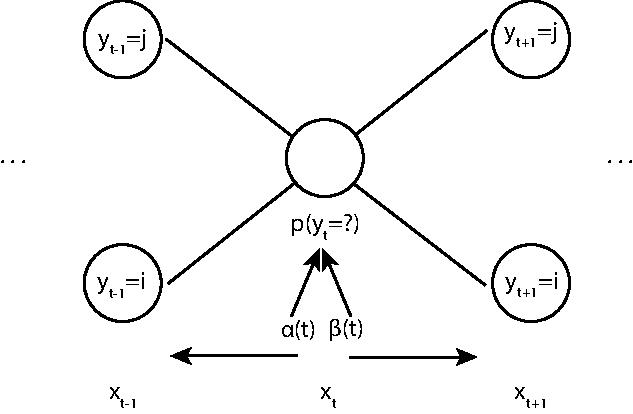
\includegraphics[width=\textwidth]{images/fwdbwd.pdf}
\caption{Information from the entire sequence $x_{1:T}$ is incorporated through the forward and backward probabilities. The formal definition of this probability is defined in equation \ref{eq:fwdbwd}}
\label{fig:fwdbwd}
\end{figure}

Figure \ref{fig:fwdbwd} illustrates how information from the entire sequence is incorporated through the forward probability, $\alpha$, and the backward probability, $\beta$, to get a \emph{smoothed probability} for $y_t = i$.

\subsection{Viterbi Algorithm}
Perhaps one of the most useful tasks for an HMM is that of decoding, or identifying the most likely parse of the sequence, $\phi_{max}$. That is, $\phi_{max}$ yields the highest joint probability $P(X,Y=\phi_{max})$. 

Mathematically, the Viterbi algorithm is very similar to the forward algorithm. Rather than taking the sum at each step in the recursion, the state transition that maximizes the probability at time $t$ is stored in a list, and then a back-trace is calculated yielding the path of maximizing hidden states.

\subsubsection{Initialization}
Calculate the probability for each state at time $t=1$, $\mu_i(t=1)$, and initialize a list with each state, $V_i(t=1)$
\begin{equation}
    \mu_i(t=1) = \max_i p(x_1|y_i)p(y_i)
\label{eq:fwdinit}
\end{equation}
$$    V_i(t=1) = i$$
\subsubsection{Induction}
Calculate the probability of being in each state $i$ at time $t$, after transitioning from state $j$ at time $t-1$, then save the largest probability $\mu_i(t)$ for each state. 
\begin{equation}
    \mu_i(t) =\max_j\left[p(x_t|y_i)p(y_i|y_j)V_j(t-1)\right]
\label{eq:fwdinduc}
\end{equation}

Then, for each state $i$, save the state transition $i\rightarrow j$ that maximized $\mu_i(t)$.  
$$V_i(t) =\argmax_j\left[p(x_t|y_i)p(y_i|y_j)V_j(t-1)\right]$$

\subsubsection{Termination}
The probability of the most likely end state is then
\begin{equation}
    P^*(t=L) = \max_i{\mu_i(t=L)}
\label{eq:fwdterm}
\end{equation}
And the back-trace for the Viterbi most likely path is initialized at the last observation $t=L$:
$$V^*(t=L) = \argmax_i{P^*(t=L)}$$
At time $t=L-1$, we then retrieve $V^*(t=L-1)$, which is the state that transitioned to the known maximizing state $V^*(t=L)$. This recursion is then repeated to the beginning of the sequence.
\begin{equation}
V^*(t-1) = \argmax_i{\mu_i(t)}
\label{eq:backtrace}    
\end{equation}

Once the list created from equation \ref{eq:backtrace} has been inverted, as it is a back-trace, the path $V^* = \phi_{max}$, which is the parse $\phi \in \Phi$ that maximizes the joint probability of the HMM. 
\subsection{Baum-Welch Algorithm}
